\documentclass{hitec}  % Your existing document class
\usepackage{lipsum}    % For dummy text
\usepackage{graphicx}  % Basic image inclusion

% FOR MINDMAPS
\usepackage{tikz}
\usetikzlibrary{mindmap, shadows} % Adds mindmap functionality, plus optional shadows

% OPTIONAL: EXTRA IMAGE CONTROL
\usepackage{wrapfig}    % Wrap text around figures
\usepackage{caption}    % Customize figure captions
\usepackage{subcaption} % Sub-figures with separate captions
\usepackage{float}      % More control over float placements

%%%%% Indent the subsections
\makeatletter
\renewcommand\subsection{\@startsection{subsection}{2}{10pt} % Indents by ~2 spaces
  {-3.25ex\@plus -1ex \@minus -.2ex} % Space before subsection
  {1.5ex \@plus .2ex}                % Space after subsection
  {\secshape\normalfont\normalsize\bfseries}}
\makeatother
%%%%% Indent the subsections END

\title{Vision and Value Workshop Report for QQQ}
\author{ZZZ}
\date{February 2025}

\begin{document}
\maketitle

% Example: Mindmap
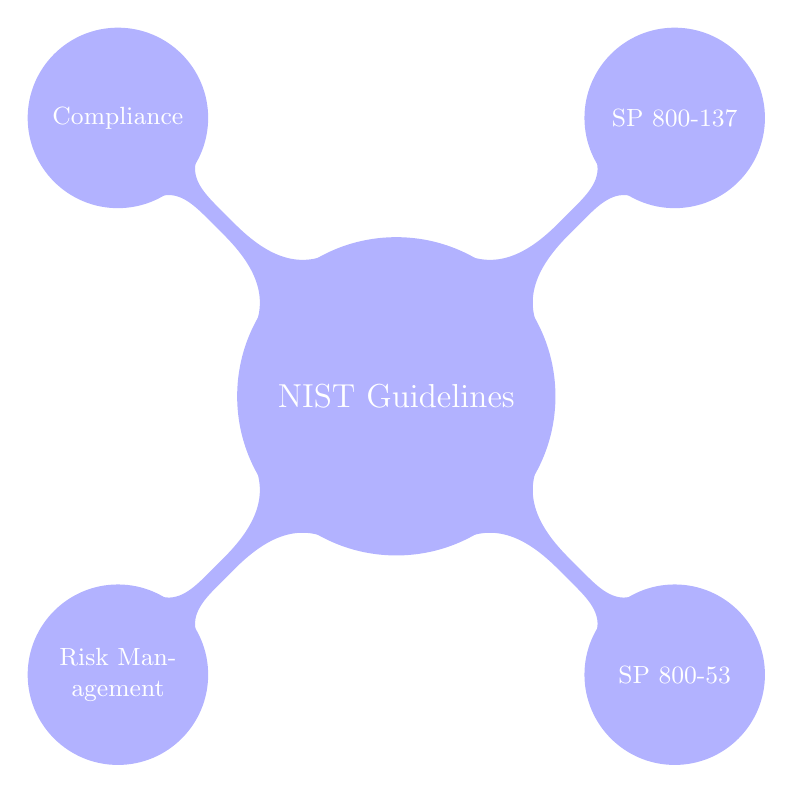
\begin{tikzpicture}
  \path[mindmap, concept color=blue!30, text=white]
    node[concept] {NIST Guidelines}
    [grow cyclic, level 1 concept/.append style={level distance=5cm,sibling angle=90}]
    child { node[concept] {Risk Management} }
    child { node[concept] {SP 800-53} }
    child { node[concept] {SP 800-137} }
    child { node[concept] {Compliance} };
\end{tikzpicture}

% Example: Inserting a figure with subfigures/wrap
\begin{wrapfigure}{r}{0.45\textwidth}
    \centering
    \includegraphics[width=0.4\textwidth]{example-image}
    \caption{Wrapped example image}
\end{wrapfigure}

\lipsum[1-2] % Dummy text to show wrapfigure usage

\end{document}
